% Provenance (never printed): cycle 4 SVT, "La planete Terre, l'environnement
% et l'action humaine": climate, its past variations and the present change,
% read from data; see sources/book1/PROVENANCE.md. Book 1, grade 9, chapter 1.
% Vocabulary guard: owns climate change (first look; Book 2 g12 re-uses it),
% global warming, temperature anomaly. The greenhouse effect and greenhouse
% gases belong to the chemistry series (grade 8): recalled in prose, never
% defined. Infrared is physics (g10): named in prose only. "Glacial period"
% and "interglacial" belong to Book 2 g12: here "the ice ages and the warmer
% times between them". Physical science only, in the IPCC's calibrated words;
% no policy.
\chapter{Het klimaat van de Aarde, vroeger en nu}\label{ch:g9:climate-past-and-present}

Als de Aarde geen lucht om zich heen had, maar evenveel zonlicht
weerkaatste als nu, zou haar oppervlak uitkomen op een gemiddelde
temperatuur van ongeveer \qty{-19}{\degreeCelsius}: bevroren \omterm{def:g2:water-on-earth:ocean}{zeeën},
bevroren land, overal. Haar werkelijke gemiddelde is ongeveer
\qty{15}{\degreeCelsius}. Het verschil, zo'n \qty{34}{\degreeCelsius},
komt van een paar gassen in de lucht, in piepkleine hoeveelheden
aanwezig, die verhinderen dat een deel van de warmte van de Aarde naar de
ruimte ontsnapt. Dit hoofdstuk gaat over deze gassen, over het \omterm{def:g5:weather-and-climate:climate}{klimaat} van
de Aarde in het verleden, en over hoe en waarom het nu verandert.
% ledger: earth:Tbb, earth:Tsurf (figdata/grade-9/climate_records.py: -19.1 and 14.9 degC, gap 34)

\begin{recall}
Het \omterm{def:g5:weather-and-climate:climate}{klimaat} van een plaats is het \omterm{def:g1:watching-the-weather:weather}{weer} dat ze gewoonlijk heeft, gemiddeld
over 30 jaar (\cref{ch:g5:weather-and-climate}). De onderste laag van de
atmosfeer, waar het \omterm{def:g1:watching-the-weather:weather}{weer} zich afspeelt, is de \omterm{def:g8:the-atmosphere:layers}{troposfeer}
(\cref{ch:g8:the-atmosphere}). IJstijden, met \omterm{def:g8:ice-on-earth:ice-sheet}{ijskappen} tot ver buiten de
\omterm{def:g3:continents-and-oceans:poles}{polen}, zijn gekomen en gegaan; het Arctische \omterm{def:g8:ice-on-earth:sea-ice}{zee-ijs} is sinds 1979
gekrompen (\cref{ch:g8:ice-on-earth}). In de scheikunde leer je dat
koolstofdioxide, methaan en waterdamp \emph{broeikasgassen} zijn: ze laten
zonlicht door maar absorberen het onzichtbare infrarode licht dat de warme
grond uitzendt, en dat is het \emph{broeikaseffect}; bij het verbranden
van steenkool, aardolie en aardgas komt koolstofdioxide vrij.
\end{recall}

\section{Het broeikaseffect en de temperatuur van de Aarde}

Zonlicht gaat door de atmosfeer en verwarmt de grond en de \omterm{def:g2:water-on-earth:ocean}{oceanen}. Zoals
elk warm voorwerp zendt het warme oppervlak op zijn beurt energie uit, als
infrarood licht dat het oog niet kan zien. Als dat allemaal naar de ruimte
ontsnapte, zou de Aarde de bevroren wereld van de eerste alinea zijn. Maar
de broeikasgassen in de lucht absorberen een groot deel van dit infrarode
licht en sturen een deel ervan terug naar beneden: het oppervlak krijgt
energie van de Zon en van de lucht erboven, en komt uit op een hogere
temperatuur.

\begin{omfigure}
\begin{tikzpicture}[font=\footnotesize, >={Stealth[length=2.4mm]}]
  % ground and atmosphere
  \fill[omLithAlluv] (0,0) rectangle (12,0.5);
  \fill[omSea!45] (0,0.5) rectangle (12,3.4);
  \node[anchor=north east, align=right] at (11.85,3.35) {atmosfeer met\\ broeikasgassen};
  \node[anchor=south east] at (11.9,0.05) {grond en oceanen};
  \node[anchor=south west] at (0.15,3.5) {ruimte};
  % Sun
  \fill[omWxSun] (1.3,5.0) circle (0.45);
  \node at (1.3,4.3) {Zon};
  % sunlight in
  \draw[->, omWxSun!80!black, line width=2.2pt] (1.7,4.6) -- (2.7,0.55)
    node[pos=0.25, right=2pt, align=left, black] {zonlicht komt binnen\\ en verwarmt het oppervlak};
  % infrared out and back
  \draw[->, omWarm, line width=1.6pt, decorate, decoration={snake, amplitude=1mm, segment length=4mm, post length=3mm}]
    (6.0,0.55) -- (6.6,2.6);
  \draw[->, omWarm, line width=1.6pt, decorate, decoration={snake, amplitude=1mm, segment length=4mm, post length=3mm}]
    (6.6,2.7) -- (7.4,5.0) node[right, align=left, black] {een deel ontsnapt\\ naar de ruimte};
  \draw[->, omWarm, line width=1.6pt, decorate, decoration={snake, amplitude=1mm, segment length=4mm, post length=3mm}]
    (6.8,2.75) -- (8.6,0.55);
  \node[align=left, anchor=west] at (8.8,1.9) {de gassen nemen\\ een deel op en\\ sturen het terug};
  \node[align=right, anchor=east] at (5.9,1.3) {het warme oppervlak\\ zendt infrarood uit};
\end{tikzpicture}

{\small Het broeikaseffect, eenvoudig (een schets). Zonder dit effect zou
het oppervlak van de Aarde gemiddeld ongeveer \qty{-19}{\degreeCelsius}
zijn; met dit effect ongeveer \qty{15}{\degreeCelsius}.}
% ledger: earth:Tbb, earth:Tsurf
\label{fig:g9:climate-past-and-present:greenhouse}
\end{omfigure}

Het broeikaseffect is natuurlijk en noodzakelijk: zonder dit effect zou er
aan het oppervlak geen vloeibaar water zijn. De vraag van dit hoofdstuk is
een andere: wat gebeurt er met de temperatuur van de Aarde als de
hoeveelheid broeikasgas in de lucht verandert?

\section{Klimaten uit het verleden}

Om het \omterm{def:g5:weather-and-climate:climate}{klimaat} van het verre verleden te lezen, boren wetenschappers in de
\omterm{def:g8:ice-on-earth:ice-sheet}{ijskappen}. Elk jaar valt er \omterm{def:g4:clouds-rain-snow:precipitation}{sneeuw} op Antarctica en Groenland, en de
zomersneeuw is een beetje anders dan de wintersneeuw. Begraven en tot ijs
samengeperst blijven de jaarlagen bewaard, de ene boven de andere, zoals
de bladzijden van een boek. Hoe dieper het ijs, hoe ouder het is.
% ledger: eo:ice-core

\begin{omfigure}
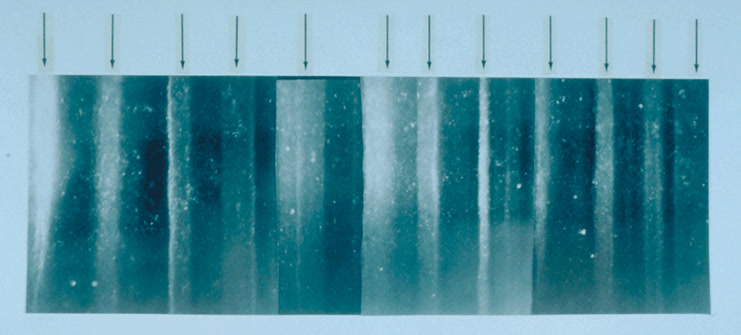
\includegraphics[width=0.78\linewidth]{images/book1/g9-gisp2-layers.jpg}

{\small Een stuk ijskern van \qty{19}{cm} lang, geboord op een diepte van
\qty{1855}{m} in de Groenlandse \omterm{def:g8:ice-on-earth:ice-sheet}{ijskap} en van onderaf belicht. De pijlen
wijzen naar de lichtere zomerlagen, tussen donkerdere winterlagen: elf
jaar \omterm{def:g4:clouds-rain-snow:precipitation}{sneeuw}. NOAA Paleoclimatology (publiek domein, via Wikimedia
Commons).}
% ledger: commons:gisp2-layers
\label{fig:g9:climate-past-and-present:ice-core}
\end{omfigure}

Een ijskern bewaart twee archieven van het verleden. De \omterm{def:g4:clouds-rain-snow:precipitation}{sneeuw} zelf
vertelt hoe koud de lucht was toen ze viel: hoe kouder de lucht, hoe
kleiner het aandeel van de zwaardere vormen van waterstof en zuurstof in
de \omterm{def:g4:clouds-rain-snow:precipitation}{sneeuw}. En terwijl \omterm{def:g4:clouds-rain-snow:precipitation}{sneeuw} tot ijs wordt samengeperst, sluiten de ruimtes
tussen de korrels zich, en worden er piepkleine belletjes lucht van die
tijd ingesloten. Wetenschappers laten deze oude lucht in het laboratorium
vrij en meten het koolstofdioxide erin.
% ledger: eo:ice-core

\begin{omfigure}
\begin{tikzpicture}
\begin{axis}[name=temp, omrecord, omage, width=13cm, height=3.9cm, xmin=0, xmax=800,
  xtick={0,100,...,800}, xticklabels={}, ylabel={temperatuur-\\ verandering ($^\circ$C)},
  ylabel style={align=center}, ymin=-11, ymax=5, ytick={-10,-5,0,5}]
  \addplot[omWarm, line width=0.7pt] table[x=age_kyr, y=temp_C] {figdata/out/grade-9-climate_records-edc.dat};
\end{axis}
\begin{axis}[at={(temp.south west)}, anchor=north west, yshift=-0.3cm, omrecord, omage,
  width=13cm, height=3.9cm, xmin=0, xmax=800, xtick={0,100,...,800},
  xlabel={duizenden jaren voor nu}, ylabel={koolstof-\\ dioxide (ppm)},
  ylabel style={align=center}, ymin=160, ymax=320, ytick={180,220,260,300}]
  \addplot[black, line width=0.7pt] table[x=age_kyr, y=co2_ppm] {figdata/out/grade-9-climate_records-icecore.dat};
\end{axis}
\end{tikzpicture}

{\small Achthonderdduizend jaar gelezen in het ijs van Antarctica. Boven:
de verandering van de luchttemperatuur op Dome~C, vergeleken met het
gemiddelde van de laatste duizend jaar (ijskern EPICA Dome~C, J.~Jouzel en
anderen, 2007). Onder: het koolstofdioxide van de lucht die in het ijs is
ingesloten, in deeltjes per miljoen (B.~Bereiter en anderen, 2015). Beide
gemiddeld over stappen van \num{2000} jaar; de tijd loopt van links
(oudst) naar rechts (nu).}
% ledger: data:edc-jouzel, data:co2-bereiter (figdata/grade-9/climate_records.py)
\label{fig:g9:climate-past-and-present:icecore}
\end{omfigure}

De twee krommen vertellen hetzelfde verhaal. Keer op keer maakten lange
koude tijden, de \omterm{def:g8:ice-on-earth:ice-age}{ijstijden}, plaats voor kortere warme tijden, en dan kwam
de kou terug. Op het koudst was de lucht boven Antarctica ongeveer
\qty{9}{\degreeCelsius} kouder dan in de laatste duizend jaar; in de
warmste tijden was ze een paar graden warmer. En het koolstofdioxide steeg
en daalde met de temperatuur, tussen ongeveer \qty{175}{ppm} in de koude
tijden en ongeveer \qty{300}{ppm} in de warme. Wij leven in een van de
warme tijden, die begon toen de laatste \omterm{def:g8:ice-on-earth:ice-age}{ijstijd} eindigde.
% ledger: data:edc-jouzel, data:co2-bereiter (figdata/grade-9/climate_records.py: edc min -9.7, max +3.6; CO2 174 to 299 ppm)

\begin{method}[Twee archieven naast elkaar lezen]
\begin{enumerate}
  \item Controleer dat de twee archieven dezelfde tijdas hebben, en in
        welke richting de tijd loopt.
  \item Kies een datum op de tijdas en lees elk archief bij die datum af.
  \item Zoek naar pieken en \omterm{def:g1:landscapes-around-us:landform}{dalen}: komen ze in beide archieven op dezelfde
        tijden?
  \item Zeg wat samen beweegt, zonder al te beslissen welke verandering de
        andere heeft veroorzaakt.
\end{enumerate}
\end{method}

\begin{example}[De laatste ijstijd in de ijskern]
Bij \num{20000} jaar voor nu (de 20 op de tijdas) staat de
temperatuurkromme op ongeveer \qty{-9}{\degreeCelsius} en het
koolstofdioxide op ongeveer \qty{190}{ppm}. In de laatste duizend jaar
ligt de temperatuurkromme dicht bij 0 en het koolstofdioxide dicht bij
\qty{280}{ppm}. Op het koudst van de laatste \omterm{def:g8:ice-on-earth:ice-age}{ijstijd} was de lucht boven
Antarctica dus ongeveer \qty{9}{\degreeCelsius} kouder, en bevatte ze
ongeveer $280 - 190 = \qty{90}{ppm}$ minder koolstofdioxide, een derde
minder.
\end{example}
% ledger: data:edc-jouzel, data:co2-bereiter (figdata/grade-9/climate_records.py: 19-21 kyr bins -9.4, 190 ppm; 1 kyr bin 278)

Nog verder terug kende de Aarde klimaten die veel warmer waren dan alle
klimaten van de laatste 800\,000 jaar. De wetenschappelijke
beoordelingen schatten dat het oppervlak van de Aarde voor het laatst
\qty{2.5}{\degreeCelsius} of meer boven zijn niveau van het eind van de
19e eeuw bleef, meer dan drie miljoen jaar geleden.
% ledger: ipcc:3myr

\section{De metingen van nu}

Sinds het eind van de 19e eeuw wordt de temperatuur elke dag gemeten op
duizenden \omterm{def:g4:clouds-rain-snow:weather-station}{weerstations} op het land en op \omterm{def:g2:water-on-earth:ocean}{zee}, met thermometers in de
schaduw. Om de hele planeet te volgen, middelen wetenschappers niet de
temperaturen zelf, die afhangen van waar elk station staat, maar hoeveel
elk station afwijkt van zijn eigen gewone waarde.
% ledger: giss:method

\begin{definition}[Temperatuuranomalie]\label{def:g9:climate-past-and-present:anomaly}
Een \emph{temperatuuranomalie}\index{temperatuuranomalie} is het verschil
tussen een temperatuur en het gemiddelde ervan over een gekozen
referentieperiode. Ze is positief als het warmer is dan dat gemiddelde, en
negatief als het kouder is.
\end{definition}

\begin{omfigure}
\begin{minipage}[c]{0.44\linewidth}\centering
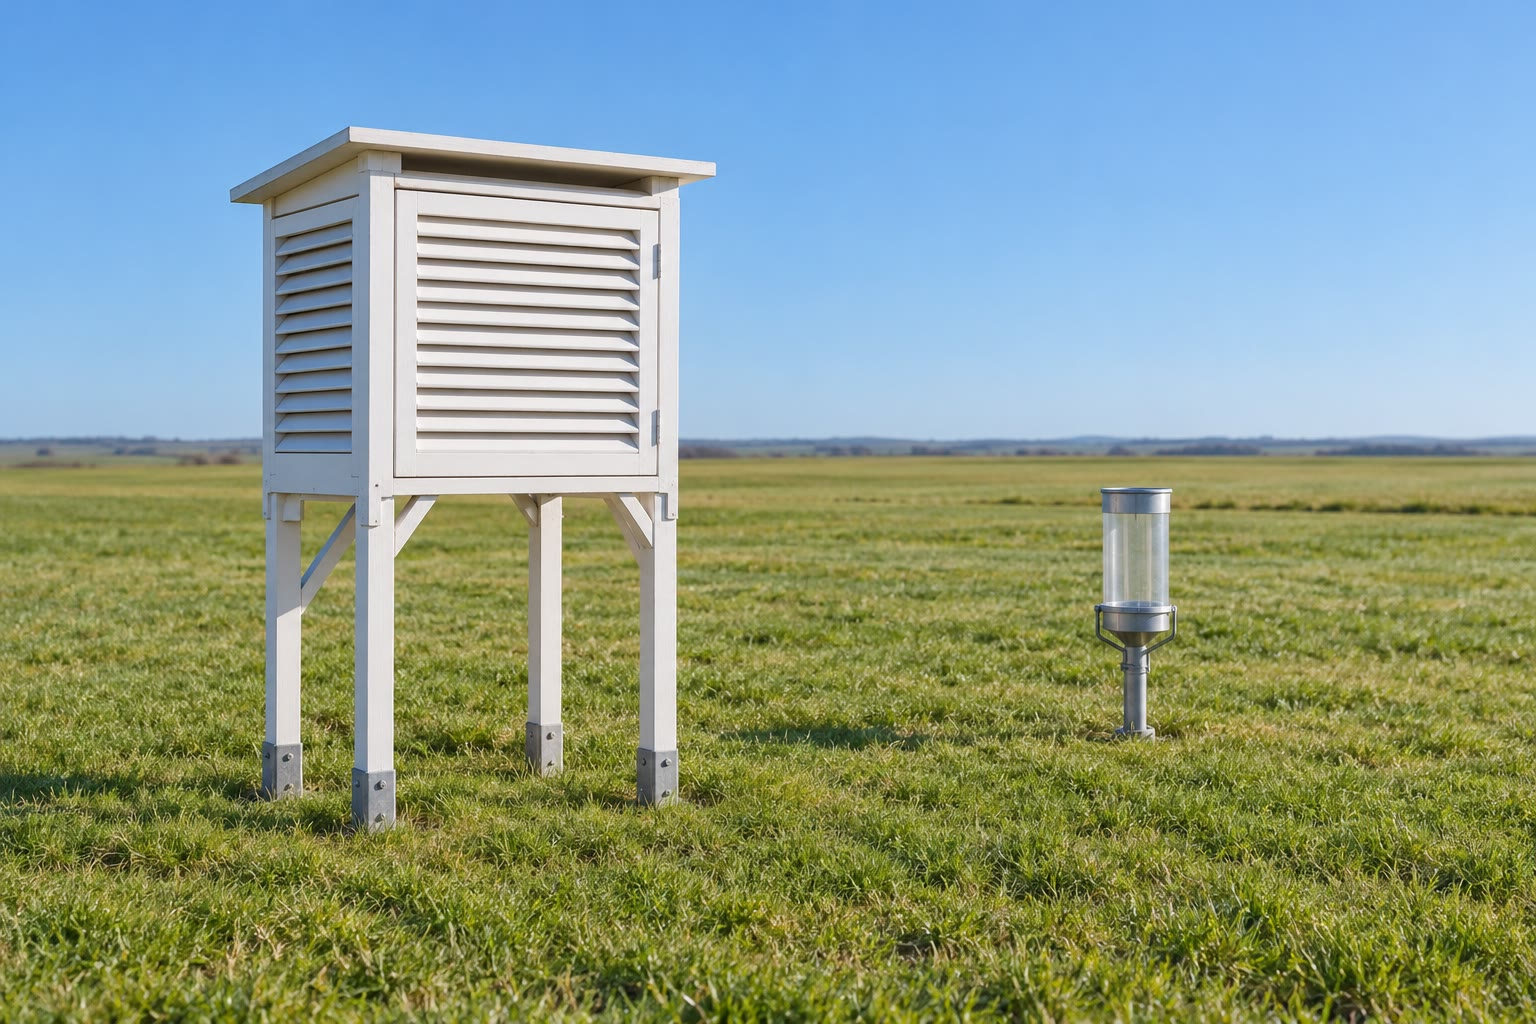
\includegraphics[width=\linewidth]{images/book1/ai/g9-weather-screen.jpg}
\end{minipage}\hfill
\begin{minipage}[c]{0.52\linewidth}\raggedright
{\small Een \omterm{def:g4:clouds-rain-snow:weather-station}{weerstation}: de witte hut op poten, met wanden van latjes,
houdt de thermometers in de schaduw terwijl de lucht erdoor stroomt;
rechts een \omterm{def:g4:clouds-rain-snow:rain-gauge}{regenmeter} (door AI gegenereerde illustratie van een algemene
scène).}
\end{minipage}
\label{fig:g9:climate-past-and-present:screen}
\end{omfigure}

Het temperatuurarchief van de NASA geeft bijvoorbeeld de anomalie van elk
jaar ten opzichte van het gemiddelde van 1951--1980, uit landstations en
uit metingen van het zeeoppervlak. Decennium per decennium gemiddeld laat
het een duidelijke stijging zien.
% ledger: giss:method, data:gistemp

\begin{omfigure}
\begin{tikzpicture}
\begin{axis}[omrecord, ybar, width=13cm, height=5.6cm, bar width=9pt,
  ymin=-0.45, ymax=1.2, ytick={-0.4,0,0.4,0.8,1.2},
  xtick=data, xticklabels={1880--89, 1890--99, 1900--09, 1910--19, 1920--29, 1930--39, 1940--49, 1950--59, 1960--69, 1970--79, 1980--89, 1990--99, 2000--09, 2010--19, 2020--25},
  x tick label style={rotate=60, anchor=east, font=\scriptsize},
  ylabel={temperatuuranomalie ($^\circ$C)}, xmajorgrids=false]
  \addplot[fill=omWarm!70, draw=black!50] table[x expr=\coordindex, y=mean_C]
    {figdata/out/grade-9-climate_records-decades.dat};
\end{axis}
\end{tikzpicture}

{\small De mondiale oppervlaktetemperatuur, decennium per decennium sinds
de jaren 1880, als anomalie ten opzichte van het gemiddelde van
1951--1980; de laatste staaf beslaat de zes jaren 2020--2025. Gegevens:
NASA GISTEMP versie~4.}
% ledger: data:gistemp (figdata/grade-9/climate_records.py)
\label{fig:g9:climate-past-and-present:decades}
\end{omfigure}

\begin{definition}[Mondiale opwarming]\label{def:g9:climate-past-and-present:global-warming}
De \emph{mondiale opwarming}\index{mondiale opwarming} is de stijging van
de gemiddelde temperatuur van het oppervlak van de Aarde als geheel, sinds
de tweede helft van de 19e eeuw.
\end{definition}

Van jaar tot jaar gaat het archief op en neer: het ene jaar kan koeler zijn
dan het vorige, omdat ook het \omterm{def:g1:watching-the-weather:weather}{weer} van een heel jaar, boven \omterm{def:g2:water-on-earth:ocean}{oceanen} en
\omterm{def:g3:continents-and-oceans:continent}{continenten}, varieert. Om een opwarming te meten, vergelijken
wetenschappers daarom gemiddelden over vele jaren, nooit twee losse jaren.

\begin{omfigure}
\begin{tikzpicture}
\begin{axis}[omrecord, width=13cm, height=5.4cm, xmin=1875, xmax=2030, ymin=-0.6, ymax=1.4,
  xtick={1880,1900,...,2020}, x tick label style={/pgf/number format/1000 sep={}},
  xlabel={jaar}, ylabel={temperatuuranomalie ($^\circ$C)},
  legend style={at={(0.2,0.97)}, anchor=north west, draw=none, fill=white, font=\footnotesize}]
  \fill[omWarm!10] (axis cs:1880,-0.6) rectangle (axis cs:1899,1.4);
  \fill[omWarm!10] (axis cs:2015,-0.6) rectangle (axis cs:2024,1.4);
  \addplot[black!70, mark=*, mark size=0.9pt, line width=0.4pt]
    table[x=year, y=anomaly_C] {figdata/out/grade-9-climate_records-annual.dat};
  \addlegendentry{elk jaar}
  \addplot[omWarm, line width=2pt] table[x=year, y=mean_C] {figdata/out/grade-9-climate_records-periods.dat};
  \addlegendentry{gemiddelde van een periode}
  \draw[dashed, black!50] (axis cs:1875,0) -- (axis cs:2030,0);
  \node[font=\scriptsize, fill=white, inner sep=1pt] at (axis cs:1889.5,0.45) {1880--1899};
  \node[font=\scriptsize, fill=white, inner sep=1pt] at (axis cs:2019.5,0.3) {2015--2024};
\end{axis}
\end{tikzpicture}

{\small De mondiale \omterm{def:g9:climate-past-and-present:anomaly}{temperatuuranomalie} van elk jaar van 1880 tot 2025
(ten opzichte van het gemiddelde van 1951--1980, stippellijn), met de
gemiddelden van twee perioden uit het probleem van dit hoofdstuk:
1880--1899 en 2015--2024. Gegevens: NASA GISTEMP versie~4.}
% ledger: data:gistemp (figdata/grade-9/climate_records.py)
\label{fig:g9:climate-past-and-present:annual}
\end{omfigure}

\begin{method}[Een opwarming tussen twee perioden meten]
\begin{enumerate}
  \item Kies twee perioden van elk minstens tien jaar, een vroege en een
        late, zodat de schommelingen van losse jaren tegen elkaar wegvallen.
  \item Middel de jaarlijkse anomalieën van elke periode.
  \item Trek het vroege gemiddelde af van het late: het resultaat is de
        opwarming tussen de twee perioden, in graden.
  \item Zeg welk archief en welke perioden je hebt gebruikt: een ander
        archief, of andere perioden, geven een iets ander getal.
\end{enumerate}
\end{method}

\begin{example}[De opwarming sinds de jaren 1970]
In het archief van de NASA zijn de anomalieën van de tien jaren 1970--1979
gemiddeld \qty{0.03}{\degreeCelsius}, en die van 2010--2019 gemiddeld
\qty{0.80}{\degreeCelsius}. De opwarming tussen deze twee decennia is
$0.80 - 0.03 = \qty{0.77}{\degreeCelsius}$, in veertig jaar: ongeveer
\qty{0.19}{\degreeCelsius} per decennium. Losse jaren, ook veertig jaar
uit elkaar, zouden heel verschillende antwoorden geven: 1976 ($-0.10$)
tegenover 2016 (1.01) geeft \qty{1.11}{\degreeCelsius}, maar 1979 (0.16)
tegenover 2011 (0.61) geeft maar \qty{0.45}{\degreeCelsius}.
\end{example}
% ledger: data:gistemp (figdata/grade-9/climate_records.py: decade_1970s 0.03, decade_2010s 0.80; annual 1976 -0.10, 2016 1.01, 1979 0.16, 2011 0.61)

Het koolstofdioxide van de lucht wordt sinds maart 1958 rechtstreeks
gemeten, in een observatorium op ongeveer \qty{3400}{m} hoogte op de
hellingen van de \omterm{def:g4:volcanoes-earthquakes-first-look:volcano}{vulkaan} Mauna Loa, op Hawaï. In 1959 was het
jaargemiddelde \qty{316}{ppm}; in 2025 had het \qty{427}{ppm} bereikt,
ver boven de \qty{300}{ppm} die het in 800\,000 jaar ijs nooit
overschreed. Het stijgt steeds sneller: met minder dan \qty{1}{ppm} per
jaar in de jaren 1960, met meer dan \qty{2.5}{ppm} per jaar in de laatste
tien jaar.
% ledger: gml:keeling, data:co2-mlo, data:co2-bereiter (figdata/grade-9/climate_records.py: 315.98, 427.35, 0.86 and 2.63 ppm/yr; ice core max 298.6)

\begin{omfigure}
\begin{tikzpicture}
\begin{axis}[omrecord, width=12cm, height=5cm, xmin=1955, xmax=2030,
  ymin=290, ymax=440, ytick={300,350,400}, xtick={1960,1970,...,2020},
  x tick label style={/pgf/number format/1000 sep={}},
  xlabel={jaar}, ylabel={koolstofdioxide (ppm)}]
  \addplot[black, line width=0.9pt, mark=*, mark size=0.8pt] table[x=year, y=co2_ppm] {figdata/out/grade-9-climate_records-co2.dat};
  \draw[dashed, omWarm] (axis cs:1955,300) -- (axis cs:2030,300);
\end{axis}
\end{tikzpicture}

{\small Het koolstofdioxide van de lucht op Mauna Loa, Hawaï,
jaargemiddelden 1959--2025 (NOAA Global Monitoring Laboratory en Scripps
Institution of Oceanography). De stippellijn bij \qty{300}{ppm} is
ongeveer het hoogste niveau dat in 800\,000 jaar Antarctisch ijs is
gevonden.}
% ledger: data:co2-mlo, data:co2-bereiter (figdata/grade-9/climate_records.py)
\label{fig:g9:climate-past-and-present:co2}
\end{omfigure}

\begin{dated}{2025}
Het jaargemiddelde van het koolstofdioxide op Mauna Loa was in 2025
\qty{427.35}{ppm}. In het archief van de NASA was 2024 het warmste jaar
sinds 1880, met een anomalie van \qty{1.28}{\degreeCelsius} ten opzichte
van 1951--1980.
% ledger: data:co2-mlo, data:gistemp (figdata/grade-9/climate_records.py)
\end{dated}

De \omterm{def:g2:water-on-earth:ocean}{zee} stijgt ook. Sinds 1993 meten satellieten de hoogte van het
zeeoppervlak over de hele aardbol: de trendlijn van hun metingen stijgt
met ongeveer \qty{3.2}{mm} per jaar, ongeveer \qty{10}{cm} in dertig jaar.
Twee dingen doen de \omterm{def:g2:water-on-earth:ocean}{zee} stijgen: water dat opwarmt zet uit, en smeltend
ijs op het land voegt water toe aan de \omterm{def:g2:water-on-earth:ocean}{oceaan}. En het ijs krimpt:
berggletsjers trekken zich bijna overal terug, en het zomerse \omterm{def:g8:ice-on-earth:sea-ice}{zee-ijs} van
het Noordpoolgebied is sinds 1979 bijna de helft van zijn uitgestrektheid
kwijtgeraakt (\cref{ch:g8:ice-on-earth}).
% ledger: data:gmsl-lsa (figdata/grade-9/climate_records.py: 3.18 mm/yr; 101 mm 1993-2024), ipcc:b1-ice, nsidc:ice-shelves, data:b1-nsidc-sea-ice

\begin{omfigure}
\begin{tikzpicture}
\begin{axis}[omrecord, width=12cm, height=4.8cm, xmin=1992, xmax=2026,
  ymin=-30, ymax=100, xtick={1995,2000,...,2025},
  x tick label style={/pgf/number format/1000 sep={}},
  xlabel={jaar}, ylabel={zeeniveau (mm)},
  legend style={at={(0.02,0.97)}, anchor=north west, draw=none, fill=white, font=\footnotesize}]
  \addplot[omCold, mark=*, mark size=1.1pt, line width=0.6pt] table[x=year, y=gmsl_mm] {figdata/out/grade-9-climate_records-sea.dat};
  \addlegendentry{jaargemiddelde}
  \addplot[omWarm, dashed, line width=0.9pt] table[x=year, y=gmsl_mm] {figdata/out/grade-9-climate_records-sea-trend.dat};
  \addlegendentry{trendlijn}
\end{axis}
\end{tikzpicture}

{\small Het mondiale gemiddelde \omterm{def:g4:world-physical-map:altitude}{zeeniveau} gemeten door satellieten,
jaargemiddelden 1993--2024, ten opzichte van een referentieniveau, en de
trendlijn ervan (NOAA Laboratory for Satellite Altimetry).}
% ledger: data:gmsl-lsa (figdata/grade-9/climate_records.py)
\label{fig:g9:climate-past-and-present:sea}
\end{omfigure}

\section{Klimaatverandering en haar oorzaken}

\begin{definition}[Klimaatverandering]\label{def:g9:climate-past-and-present:climate-change}
\emph{Klimaatverandering}\index{klimaatverandering} is een verandering van
het \omterm{def:g5:weather-and-climate:climate}{klimaat} van de Aarde, of van een gebied, die tientallen jaren of
langer aanhoudt: een verandering van de gemiddelde temperatuur, de \omterm{def:g4:clouds-rain-snow:precipitation}{regen},
de winden of het ijs, niet maar één ongewoon seizoen.
\end{definition}

Het \omterm{def:g5:weather-and-climate:climate}{klimaat} is altijd veranderd, zoals de ijskernen laten zien. Wat nieuw
is, is de snelheid van de huidige verandering, en haar oorzaak.
Wetenschappers van over de hele wereld beoordelen regelmatig wat er over
het \omterm{def:g5:weather-and-climate:climate}{klimaat} is gepubliceerd, in de rapporten van het Intergovernmental
Panel on Climate Change (IPCC), het klimaatpanel van de Verenigde Naties.
De rapporten wegen hoe zeker elke uitspraak is, met zorgvuldig gekozen
woorden.

In deze rapporten heeft elk van de woorden hieronder een vaste betekenis:
de kans op 100 dat de uitspraak waar is.

\begin{center}
{\small
\begin{tabular}{|l|c||l|c|}
\hline
\emph{vrijwel zeker} & 99 tot 100 & \emph{waarschijnlijk} & 66 tot 100 \\
\emph{uiterst waarschijnlijk} & 95 tot 100 & \emph{even waarschijnlijk als niet} & 33 tot 66 \\
\emph{zeer waarschijnlijk} & 90 tot 100 & \emph{onwaarschijnlijk} & 0 tot 33 \\
\hline
\end{tabular}}
\end{center}
% ledger: ipcc:likelihood

\noindent Een paar uitspraken dragen geen van deze woorden: ze worden als
feiten gegeven, zoals ``het is \emph{ondubbelzinnig}''. Let bij een
nieuwsbericht over het \omterm{def:g5:weather-and-climate:climate}{klimaat} op deze woorden, en kijk welke het bericht
houdt en welke het weglaat.
% ledger: ipcc:unequivocal

Het rapport dat in 2021 werd gepubliceerd, stelt het volgende.
\begin{itemize}
  \item Het is \emph{ondubbelzinnig} dat menselijke invloed de atmosfeer,
        de \omterm{def:g2:water-on-earth:ocean}{oceaan} en het land heeft opgewarmd.
  \item De mondiale oppervlaktetemperatuur van 2011--2020 lag ongeveer
        \qty{1.1}{\degreeCelsius} hoger dan in 1850--1900, en elk van de
        laatste vier decennia was warmer dan elk decennium ervoor sinds
        1850.
  \item De \emph{waarschijnlijke} door de mens veroorzaakte opwarming van
        1850--1900 tot 2010--2019 is 0.8 tot \qty{1.3}{\degreeCelsius},
        met een beste schatting van \qty{1.07}{\degreeCelsius}: ongeveer
        de hele waargenomen opwarming. Natuurlijke oorzaken samen
        veranderden de temperatuur met maar $-0.1$ tot $+\qty{0.1}{\degreeCelsius}$.
  \item Het koolstofdioxide van de lucht was in 2019 hoger dan op enig
        moment in minstens twee miljoen jaar (\emph{hoge mate van
        vertrouwen}); het was sinds 1750 met 47~\% gestegen.
  \item Menselijke invloed is \emph{zeer waarschijnlijk} de belangrijkste
        oorzaak van het terugtrekken van de \omterm{def:g8:ice-on-earth:glacier}{gletsjers} sinds de jaren 1990
        en van het krimpen van het Arctische \omterm{def:g8:ice-on-earth:sea-ice}{zee-ijs}; en \emph{zeer
        waarschijnlijk} de belangrijkste oorzaak van de stijging van de
        \omterm{def:g2:water-on-earth:ocean}{zee} sinds minstens 1971.
\end{itemize}
% ledger: ipcc:unequivocal, ipcc:gsat-2011-2020, ipcc:decades, ipcc:attribution, ipcc:co2-2myr, ipcc:b1-ice, ipcc:sea-level-obs

\begin{history}[De curve van Charles David Keeling]
In maart 1958 begon een jonge scheikundige van het Scripps Institution of
Oceanography, Charles David Keeling, het koolstofdioxide van de lucht te
meten op de Mauna Loa, hoog boven de \omterm{def:g2:water-on-earth:ocean}{zee} en ver van elke stad. Zijn
metingen gaan sindsdien door: ze vormen het langste archief van
koolstofdioxide dat rechtstreeks in de lucht is gemeten, en de curve die
ze tekenen, jaar na jaar stijgend, draagt zijn naam, de
\emph{Keelingcurve}.
% ledger: gml:keeling
\end{history}

Waarom volgt de opwarming het koolstofdioxide? Bij het verbranden van
steenkool, aardolie en aardgas komt koolstofdioxide vrij; meer
koolstofdioxide in de lucht betekent dat meer van het infrarode licht dat
het oppervlak uitzendt, wordt geabsorbeerd en teruggestuurd, en het
oppervlak warmt op. Waterdamp, methaan en de andere broeikasgassen dragen
bij aan het effect. Verleden en heden zijn het eens: in de ijskernen
zoals in de metingen van nu stijgen en \omterm{def:g1:landscapes-around-us:landform}{dalen} de temperatuur van de Aarde
en haar koolstofdioxide samen.
% ledger: ipcc:attribution, ipcc:co2-2myr

\section{Oefeningen}

\begin{exercise}[$\star$]\label{exo:g9:climate-past-and-present:1}
% ledger: earth:Tbb, earth:Tsurf
(a) Wat zou de gemiddelde temperatuur van het oppervlak van de Aarde zijn
zonder het broeikaseffect? (b) En met het broeikaseffect? (c) Hoeveel
graden warmt het broeikaseffect het oppervlak op? (d) Noem twee
broeikasgassen.
\end{exercise}

\begin{exercise}[$\star$]\label{exo:g9:climate-past-and-present:2}
\omterm{def:g1:watching-the-weather:weather}{Weer} of \omterm{def:g5:weather-and-climate:climate}{klimaat}? (a) Gisteren heeft het de hele dag geregend. (b) De
zomers in dit gebied zijn heet en droog. (c) De jaren 2010 waren
wereldwijd warmer dan de jaren 1980. (d) Volgende week wordt het koud.
\end{exercise}

\begin{exercise}[$\star$]\label{exo:g9:climate-past-and-present:3}
% ledger: commons:gisp2-layers
Kijk naar de foto van het stuk ijskern. (a) Hoe lang is het stuk, en
hoeveel jaar \omterm{def:g4:clouds-rain-snow:precipitation}{sneeuw} bevat het? (b) Bereken de gemiddelde dikte van één
jaarlaag, in centimeter. (c) Waarom is het diepste ijs van een \omterm{def:g8:ice-on-earth:ice-sheet}{ijskap} het
oudste?
\end{exercise}

\begin{exercise}[$\star$]\label{exo:g9:climate-past-and-present:4}
De gemiddelde julitemperatuur van een stad over 1991--2020 is
\qty{21.0}{\degreeCelsius}. Geef de \omterm{def:g9:climate-past-and-present:anomaly}{temperatuuranomalie} van een juli met
een gemiddelde van (a) \qty{22.4}{\degreeCelsius};
(b) \qty{20.3}{\degreeCelsius}; (c) \qty{21.0}{\degreeCelsius}. (d) Wat
betekent een negatieve anomalie?
\end{exercise}

\begin{exercise}[$\star\star$]\label{exo:g9:climate-past-and-present:5}
% ledger: data:gistemp (figdata/grade-9/climate_records.py)
Gebruik het staafdiagram van de decennia. (a) Welke decennia waren kouder
dan het gemiddelde van 1951--1980? (b) Lees de anomalie af van de jaren
1980 en van de jaren 2010. (c) Hoeveel is de anomalie tussen deze twee
decennia gegroeid? (d) Is de stijging over het hele archief gelijkmatig
van het ene decennium naar het volgende?
\end{exercise}

\begin{exercise}[$\star\star$]\label{exo:g9:climate-past-and-present:6}
% ledger: data:co2-mlo (figdata/grade-9/climate_records.py)
Op Mauna Loa was het jaargemiddelde van het koolstofdioxide
\qty{315.98}{ppm} in 1959, \qty{324.62}{ppm} in 1969, \qty{401.01}{ppm}
in 2015 en \qty{427.35}{ppm} in 2025. (a) Wat was de gemiddelde stijging
per jaar van 1959 tot 1969? (b) Van 2015 tot 2025? (c) Hoeveel keer
sneller was de stijging in de tweede periode? (d) Met hoeveel procent is
het koolstofdioxide van 1959 tot 2025 gegroeid?
\end{exercise}

\begin{exercise}[$\star\star$]\label{exo:g9:climate-past-and-present:7}
% ledger: data:edc-jouzel, data:co2-bereiter
Gebruik het archief van 800\,000 jaar. (a) Schrijf 800\,000 jaar in de
wetenschappelijke notatie. (b) Ongeveer hoe lang geleden was het, voor
onze eigen warme tijd, voor het laatst zo warm als nu? (c) Welk
koolstofdioxidegehalte had de lucht toen? (d) Stijgen en \omterm{def:g1:landscapes-around-us:landform}{dalen} de
temperatuur en het koolstofdioxide op dezelfde momenten?
\end{exercise}

\begin{exercise}[$\star\star$]\label{exo:g9:climate-past-and-present:8}
% ledger: data:gmsl-lsa (figdata/grade-9/climate_records.py)
De \omterm{def:g2:water-on-earth:ocean}{zee} stijgt met ongeveer \qty{3.2}{mm} per jaar. (a) Hoeveel is dat in
10 jaar, in centimeter? (b) Als dit tempo aanhield, hoeveel zou de \omterm{def:g2:water-on-earth:ocean}{zee} dan
tussen 2025 en 2100 stijgen? (c) Noem twee redenen waarom de \omterm{def:g2:water-on-earth:ocean}{zee} stijgt.
(d) Doet het smelten van het Arctische \omterm{def:g8:ice-on-earth:sea-ice}{zee-ijs} de \omterm{def:g2:water-on-earth:ocean}{zee} stijgen? Leg uit.
\end{exercise}

\begin{exercise}[$\star\star$]\label{exo:g9:climate-past-and-present:9}
% ledger: ipcc:likelihood
Hoeveel kansen op 100 heeft elke uitspraak, in de woorden van het IPCC,
minstens om waar te zijn? (a) ``Het is \emph{zeer waarschijnlijk}\ldots''
(b) ``Het is \emph{waarschijnlijk}\ldots'' (c) ``Het is \emph{vrijwel
zeker}\ldots'' (d) Een krant schrijft ``wetenschappers zijn er zeker van
dat'' over een uitspraak die het rapport \emph{waarschijnlijk} noemt. Wat
is er fout?
\end{exercise}

\begin{exercise}[$\star\star$]\label{exo:g9:climate-past-and-present:10}
Een vriend zegt: ``Deze winter was waar ik woon de koudste in tien jaar,
dus de Aarde warmt niet op.'' Leg met de woorden \emph{weer},
\emph{\omterm{def:g5:weather-and-climate:climate}{klimaat}} en \emph{mondiaal} uit waarom deze redenering niet klopt.
\end{exercise}

\begin{exercise}[$\star\star\star$]\label{exo:g9:climate-past-and-present:11}
% ledger: data:co2-bereiter, data:co2-mlo, ipcc:co2-2myr, ipcc:erf-2xco2
Op het koudst van de laatste \omterm{def:g8:ice-on-earth:ice-age}{ijstijd}, ongeveer $2 \times 10^4$ jaar
geleden, bevatte de lucht ongeveer \qty{190}{ppm} koolstofdioxide; vlak
voor het industriële tijdperk ongeveer \qty{280}{ppm}; in 2025 ongeveer
\qty{427}{ppm}. (a) Hoeveel steeg het koolstofdioxide van de \omterm{def:g8:ice-on-earth:ice-age}{ijstijd} tot
het industriële tijdperk, en in hoeveel jaar? (b) Hoeveel steeg het van
het industriële tijdperk tot 2025? Neem 1750 als begin van het
industriële tijdperk. (c) Vergelijk de twee stijgingen: in grootte, en in
gemiddeld tempo per jaar, met de wetenschappelijke notatie. (d) Wat zegt
het IPCC over het koolstofdioxidegehalte van nu vergeleken met het
verleden?
\end{exercise}

\begin{exercise}[$\star\star\star$]\label{exo:g9:climate-past-and-present:12}
% ledger: ipcc:attribution, ipcc:observed-2010-2019
Het rapport van het IPCC geeft de waargenomen opwarming van 1850--1900 tot
2010--2019 als ongeveer \qty{1.06}{\degreeCelsius}, en de door de mens
veroorzaakte opwarming als \emph{waarschijnlijk} 0.8 tot
\qty{1.3}{\degreeCelsius} (beste schatting \qty{1.07}{\degreeCelsius});
de natuurlijke oorzaken samen worden gegeven als
$-0.1$ tot $+\qty{0.1}{\degreeCelsius}$. (a) Vergelijk de beste schatting
van de door de mens veroorzaakte opwarming met de waargenomen opwarming.
(b) Zouden natuurlijke oorzaken alleen de waargenomen opwarming kunnen
verklaren? Leg uit. (c) Wat betekent \emph{waarschijnlijk} in deze zin?
\end{exercise}

\section{Probleem: De thermometer van de planeet}

\begin{problem}[{Weekendprobleem --- de opwarming van de Aarde wordt
berekend uit het temperatuurarchief van de NASA, en dan naast het
koolstofdioxide en de zee gelegd}]
\label{pb:g9:climate-past-and-present:1}
% ledger: data:gistemp, data:co2-mlo, data:gmsl-lsa, ipcc:gsat-2011-2020 (figdata/grade-9/climate_records.py)
De tabel geeft de mondiale \omterm{def:g9:climate-past-and-present:anomaly}{temperatuuranomalie} van het archief van de NASA
(ten opzichte van het gemiddelde van 1951--1980) voor enkele groepen
jaren, en andere archieven uit het hoofdstuk.

\begin{center}
{\small
\begin{tabular}{|l|c|}
\hline
gemiddelde anomalie, 1880--1899 & \qty{-0.22}{\degreeCelsius} \\
gemiddelde anomalie, 1951--1980 & \qty{0.00}{\degreeCelsius} \\
gemiddelde anomalie, 2015--2024 & \qty{0.98}{\degreeCelsius} \\
koolstofdioxide op Mauna Loa, 1959 / 2025 & \qty{316}{ppm} / \qty{427}{ppm} \\
trend van het \omterm{def:g4:world-physical-map:altitude}{zeeniveau} volgens satellieten, sinds 1993 & \qty{3.2}{mm} per jaar \\
\hline
\end{tabular}}
\end{center}

\noindent\textbf{Deel I --- De decennia.}\par\nopagebreak
\begin{enumerate}[beginpenalty=10000]
  \item Waarom is de anomalie van 1951--1980 precies nul?
  \item Was 1880--1899 warmer of kouder dan 1951--1980? Hoeveel?
  \item Was 2015--2024 warmer of kouder dan 1951--1980? Hoeveel?
  \item Bereken de opwarming van 2015--2024 ten opzichte van 1880--1899.
\end{enumerate}

\noindent\textbf{Deel II --- Het koolstofdioxide.}\par\nopagebreak
\begin{enumerate}[resume, beginpenalty=10000]
  \item Met hoeveel ppm is het koolstofdioxide tussen 1959 en 2025
        gestegen?
  \item Met welk percentage van zijn waarde van 1959?
  \item In de ijskernen kwam het koolstofdioxide in 800\,000 jaar nooit
        boven ongeveer \qty{300}{ppm}. Hoeveel ligt de waarde van 2025
        daarboven?
  \item Leg in twee zinnen uit hoe meer koolstofdioxide in de lucht het
        oppervlak opwarmt.
\end{enumerate}

\noindent\textbf{Deel III --- De zee.}\par\nopagebreak
\begin{enumerate}[resume, beginpenalty=10000]
  \item Hoeveel is de \omterm{def:g2:water-on-earth:ocean}{zee} van 1993 tot 2025 gestegen met het tempo van de
        tabel, in centimeter?
  \item Noem de twee oorzaken van deze stijging.
  \item Het IPCC geeft de opwarming van 2011--2020 ten opzichte van
        1850--1900 als ongeveer \qty{1.09}{\degreeCelsius}. Is je antwoord
        op vraag~4 van dezelfde grootte? Geef één reden waarom de twee
        getallen een beetje verschillen.
  \item Schrijf de zin die een wetenschapsjournalist zou kunnen drukken:
        ``Sinds het eind van de 19e eeuw is het oppervlak van de Aarde
        opgewarmd met ongeveer \ldots''
\end{enumerate}
\end{problem}
